\documentclass[12pt]{article}
\usepackage{uwyo_report} % loads in all the specific formatting
\usepackage{amsmath}
\usepackage{amssymb}
\usepackage{float}
\usepackage{multicol}
\setlength{\multicolsep}{6.0pt plus 2.0pt minus 1.5pt}%


% if you want other packages, put them here

% macro for typesetting the word BibTeX
\def\BibTeX{{\rm B\kern-.05em{\sc i\kern-.025em b}\kern-.08em
   T\kern-.1667em\lower.7ex\hbox{E}\kern-.125emX}}


\begin{document}

\title{EE 5450  Project 02: Convolution Neural Network Classification of the Animals Data Set}

\author{David R. Mohler}

%\date{December 7, 1941}

\maketitle

\section{Introduction} 
The rebirth of Neural Networks (NNs) and Machine Learning (ML) has offered revolutionary approaches to intelligent tasks previously unattainable in the field of image processing and computer vision. A major area of research focus continues to be the classification of images. Image classification through classical means of image processing tend to suffer due to problems with the wide variance in images to be classified 
\begin{figure}[h]
	\centering % must do this or your figure won't be centered
	\captionsetup{justification=centering}
	\begin{minipage}{0.33\textwidth}
		\centering % must do this or your figure won't be centered
		\includegraphics[width=1\textwidth]{cats_00033.jpg}
	\end{minipage}\hfill
	\begin{minipage}{0.33\textwidth}
		\centering % must do this or your figure won't be centered
		\includegraphics[width=1\textwidth]{dogs_00013.jpg}
	\end{minipage}\hfill
	\begin{minipage}{0.33\textwidth}
		\centering % must do this or your figure won't be centered
		\includegraphics[width=1\textwidth]{panda_00082.jpg}
	\end{minipage}\hfill
\end{figure}

\section{Methods and Results}


\subsection{ShallowNet}
For baseline comparisons we will use the code provided by Dr. Rosebrock \cite{rosebrock} which is a simplistic implementation of a Convolutional Neural Network designed with the goal of classification of images in to any of the three given animal categories. The basic structure of Rosebrock's network consists of:
\begin{center}
	\pc{INPUT => CONV => RELU => FC => SOFTMAX} \\
\end{center}
Even with the most basic of implementations, the network is able to provide a respectable first attempt at the classification of the images. As seen in Table \ref{SNR}, the network achieves an average accuracy $66\%$. Given that with three classes the network has a $33\%$ probability of randomly selecting the correct class, this is a decent first attempt. Using this as a lower bound we proceed to implement a number of other techniques that are common in CNN architectures in order to improve the performance of the network overall. 
\begin{figure}[h]
	\centering % must do this or your figure won't be centered
	\captionsetup{justification=centering}
	\begin{minipage}{0.5\textwidth}
		\centering % must do this or your figure won't be centered
		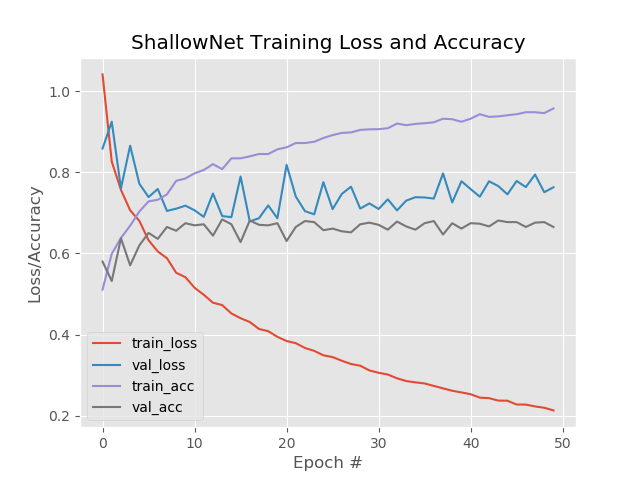
\includegraphics[width=1\textwidth]{BaselineResults_ShallowNet_opt-SGD.png}
		\caption{ShallowNet Accuracy} \label{SN}
	\end{minipage}\hfill
	\begin{minipage}{0.5\textwidth}
		\begin{center}
			\begin{tabular}[5pt]{| c| c| c| c|c|}
				\hline
				& Precision & Recall & F1-Score & Support \\[0.5ex] 
				\hline 	
				Cat   &    0.64	&0.57&	0.6&	262\\ \hline 
				Dog    &   0.57&	0.58&	0.58&	249\\ \hline 
				Panda   &   0.79&	0.86&	0.82&	239	\\ \hline 
				Avg/Total  &     0.66 &	0.67 &	0.66 &	750\\ \hline 
				
			\end{tabular}
			\captionof{table}{ShallowNet Results}\label{SNR}
		\end{center}	
	\end{minipage}
\end{figure}

\subsection{MohlerNet2}

The initial modification to the original network lies in the expansion of the architecture to incorporate key elements of CNNs, such as pooling layers and incorporation of neuron dropout prior to the fully connected layer. The general architecture of \textbf{``\pc{MohlerNet2}''} is as follows: 
\begin{center}
	\pc{INPUT => CONV => CONV => MAXPOOL => DROPOUT(0.5) => FC => SOFTMAX} \\
\end{center}
Using the classical stochastic gradient descent approach to the optimization of the network we were able to see an immediate and reproducible increase in the ability of the network to accurately classify the three categories of animal images.  From Table \ref{MNR}, it can be seen that the inclusion of the additional convolutional layer, pooling, and dropout was able to provide a $6\%$ increase in the accuracy of the network. As a more objective measure of the algorithm we can view the F-1 score for each tested network. The F-1 score captures information regarding the false positives and false negatives in the classification process, this gives a more objective view from algorithm to algorithm . From this we can also see a similar increase in F-1 score between the original ShallowNet implementation and the first implementation of MohlerNet (MohlerNet2). 
%\begin{equation}\label{NPI}
%N^j\Pi^{pj} = [(X_o^{jT}\otimes I_3)-(X_o^{jT}\otimes \chi^{pj}e_3^T)]\Pi^S = 0
%\end{equation}
\begin{figure}[h]
	\centering % must do this or your figure won't be centered
	\captionsetup{justification=centering}
	\begin{minipage}{0.5\textwidth}
		\centering % must do this or your figure won't be centered
		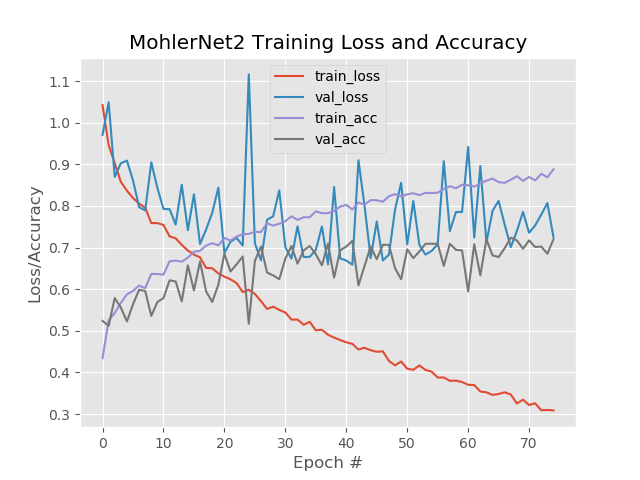
\includegraphics[width=1\textwidth]{MohlerNet2_opt-SGD_KEEP.png}
		\caption{MohlerNet2 Accuracy, Learning Rate:0.01} \label{MN2}
	\end{minipage}\hfill
	\begin{minipage}{0.5\textwidth}
		\begin{center}
			\begin{tabular}[5pt]{| c| c| c| c|c|}
				\hline
					& Precision & Recall & F1-Score & Support \\[0.5ex] 
				\hline 	
				 Cat   &    0.67  &    0.75   &   0.71   &    262\\ \hline 
				 Dog    &   0.64    &  0.60   &   0.62   &    249\\ \hline 
				 Panda   &    0.88   &  0.82 &     0.85  &     239\\ \hline 
				 Avg/Total  &     0.72    &  0.72 &     0.72    &   750\\ \hline 

			\end{tabular}
			\captionof{table}{MohlerNet2 Classification Results}\label{MNR}
		\end{center}	
	\end{minipage}
\end{figure}



\begin{figure}[h]
	\centering % must do this or your figure won't be centered
	\captionsetup{justification=centering}
	\begin{minipage}{0.5\textwidth}
		\centering % must do this or your figure won't be centered
		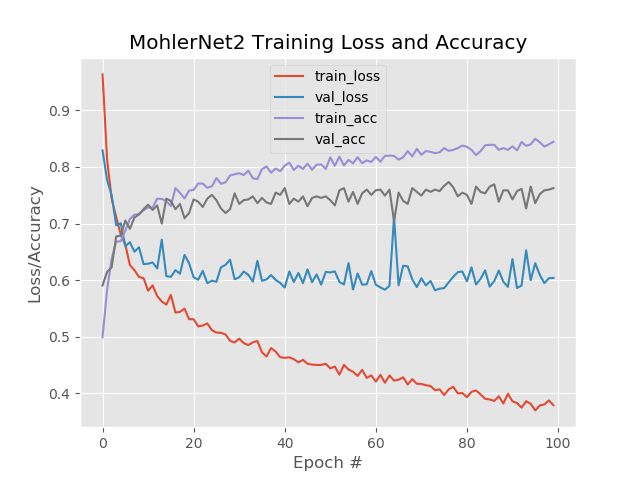
\includegraphics[width=1\textwidth]{MohlerNet2_opt-AdaGradAugment_KEEP.png}
		\caption{MohlerNet2 with Data Augmentation Accuracy, AdaGrad Optimized} \label{MN2Aug}
	\end{minipage}\hfill
	\begin{minipage}{0.5\textwidth}
		\begin{center}
			\begin{tabular}[5pt]{| c| c| c| c|c|}
				\hline
				& Precision & Recall & F1-Score & Support \\[0.5ex] 
				\hline 	
				Cat   &    0.75&	0.66&	0.71&	262\\ \hline 
				Dog    &   0.69&	0.7&	0.69&	249    \\ \hline 
				Panda   &   0.84&	0.93&	0.89&	239    \\ \hline 
				Avg/Total  &    0.76&	0.76&	0.76&	750\\ \hline 
				
			\end{tabular}
			\captionof{table}{MohlerNet2 with Data Augmentation Results}\label{MN2RAug}
		\end{center}	
	\end{minipage}
\end{figure}

\subsection{MohlerNet3}

\begin{center}
	\pc{INPUT => [CONV => MAXPOOL]*2 => CONV*3 => MAXPOOL => DROPOUT(0.5) => FC => SOFTMAX} \\
\end{center}


\begin{figure}[h]
	\centering % must do this or your figure won't be centered
	\captionsetup{justification=centering}
	\begin{minipage}{0.5\textwidth}
		\centering % must do this or your figure won't be centered
		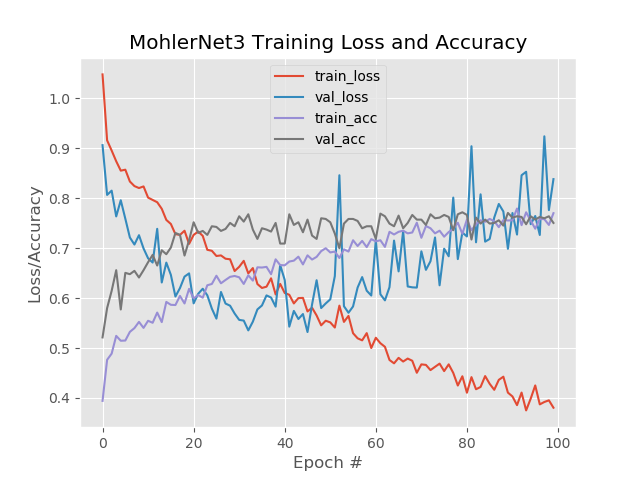
\includegraphics[width=1\textwidth]{MohlerNet3_opt-AdamaxAugmented_KEEP.png}
		\caption{MohlerNet3 with Data Augmentation Accuracy, AdaMax Optimized} \label{MN3Aug}
	\end{minipage}\hfill
	\begin{minipage}{0.5\textwidth}
		\begin{center}
			\begin{tabular}[5pt]{| c| c| c| c|c|}
				\hline
				& Precision & Recall & F1-Score & Support \\[0.5ex] 
				\hline 	
				Cat   &    0.81&      0.58 &     0.68  &     262\\ \hline 
				Dog    &   0.62 &     0.78 &     0.69 &      249    \\ \hline 
				Panda   &   0.88&      0.91  &    0.89  &     239   \\ \hline 
				Avg/Total  &    0.77 &     0.75   &   0.75   &    750\\ \hline 
				
			\end{tabular}
			\captionof{table}{MohlerNet3 with Data Augmentation Results}\label{MN2RAug}
		\end{center}	
	\end{minipage}
\end{figure}


\section{Conclusions}


\appendix % this command sets sectioning command to the appendix format
% uncomment the next line to start on a fresh page



\section{Code Listings}\label{code}

% input the file containing the code
%\lstinputlisting[caption={Top level implementation for Monocular Calibration and Pose Estimation},label={proj}]{MonoPose.m}
%\lstinputlisting[caption={QR Decomp Based Algorithm Implementation},label={alg}]{MonoPoseQR.m} 
%\lstinputlisting[caption={Rearranged QR Decomposition (Credit: Dr. John McInroy)},label={qrCom}]{qrCommute.m}


%% The commands below automatically generate the References section
%% using the ``sample_bib'' file I've given you.

\newpage  % start a new page
\bibliographystyle{ieeetr}
\bibliography{Proj2}

\end{document} % always the last line of your document file
